% Gemini theme
% https://github.com/anishathalye/gemini

\documentclass[final]{beamer}

% ====================
% Packages
% ====================

\usepackage[T1]{fontenc}
\usepackage{lmodern}
\usepackage[size=custom,width=91.44,height=121.92,scale=1.0]{beamerposter}
\usetheme{gemini}
\usecolortheme{labsix}
\usepackage{graphicx}
\usepackage{booktabs}
\usepackage{tikz}
\usepackage{pgfplots}
\pgfplotsset{compat=1.14}
\usepackage{anyfontsize}

% ====================
% Lengths
% ====================

% If you have N columns, choose \sepwidth and \colwidth such that
% (N+1)*\sepwidth + N*\colwidth = \paperwidth
\newlength{\sepwidth}
\newlength{\colwidth}
\setlength{\sepwidth}{0.025\paperwidth}
\setlength{\colwidth}{0.3\paperwidth}

\newcommand{\separatorcolumn}{\begin{column}{\sepwidth}\end{column}}

% ====================
% Title
% ====================

\title{\textsc{Multivariate Downscaling over Southern Quebec using a Probabilistic UNet}}

\author{Maryam Alipourhajiagha \inst{1} \and P.-L. Lemaire \inst{1} \and Julie Carreau \inst{1} \and Youssef Diouane \inst{1}}

\institute[shortinst]{\inst{1} Polytechnique Montréal}

% ====================
% Footer (optional)
% ====================

\footercontent{
  \href{https://github.com/pierrelouislemaire/prob-unet-mds}{github.com/pierrelouislemaire} \hfill
  Ouranos Symposium - January 2025 \hfill
  firstname.lastname@polymtl.ca}

% ====================
% Logo (optional)
% ====================

% use this to include logos on the left and/or right side of the header:
\logoright{
\includegraphics[height=7cm]{logo/ouranos_logo_vertical_couleur.pdf}}
\logoleft{
\includegraphics[height=7cm]{logo/Polytechnique_signature-CMYK-gauche_FR.pdf}}

% ====================
% Body
% ====================

\begin{document}

\begin{frame}[t]
\begin{columns}[t]
\separatorcolumn

\begin{column}{\colwidth}

  \begin{block}{\textsc{Motivation and Objective}}

    High-resolution climate simulations are essential for studying and mitigating the impacts of climate-related hazards. However, \textbf{Regional Climate Models (RCMs) come with prohibitive computational costs}, limiting the use of high-resolution climate data. \medbreak

    \noindent We explore the application of a \textbf{UNet architecture} to simultaneously downscale precipitation and temperature \textbf{without incorporating additional features}. Accurately predicting precipitation extremes and capturing fine-scale spatial patterns remain significant challenges. To address this, \textbf{we experiment with a probabilistic approach} inspired by recent advancements in generative models. The probabilistic UNet should offer the added benefit of \textbf{simplicity} while enhancing predictive performance.


  \end{block}
  
 \setbeamerfont{itemize/enumerate body}{size=\Large} % Adjust font size for the body
 \setbeamerfont{itemize/enumerate subbody}{size=\Large} % Adjust font size for subitems
  \begin{block}{\textsc{Dataset}}

    \begin{figure}
        \centering
        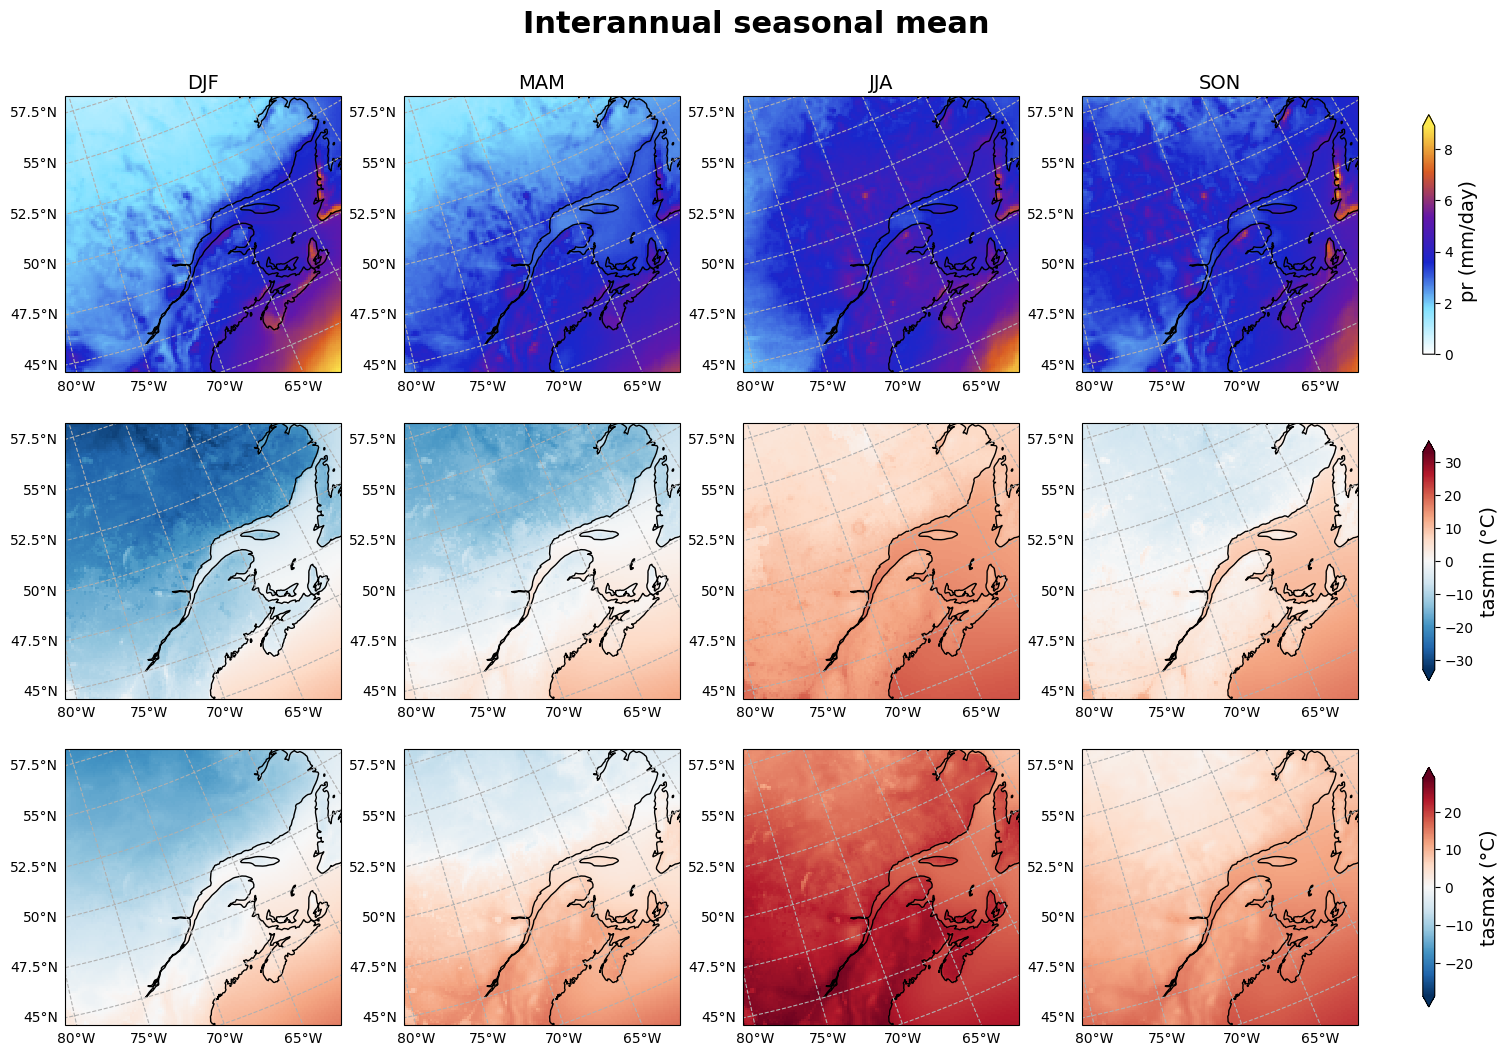
\includegraphics[width=\linewidth]{img/data.png}
    \end{figure}

    We use the Canadian Regional Climate Model Large Ensemble (CRCM5-LE), also known as \textbf{ClimEx} \cite{leduc2019climex}, which consists of dynamically downscaled simulations from the global climate model \textbf{CanESM2 50-members initial-conditions large ensemble (CanESM2-LE)}. \medbreak
    
    \noindent We focus on \textbf{Southern Quebec} and Canadian Maritime provinces. 

    
    
  \end{block}

  \begin{block}{\textsc{Training Framework}}

    \begin{figure}
      \centering
      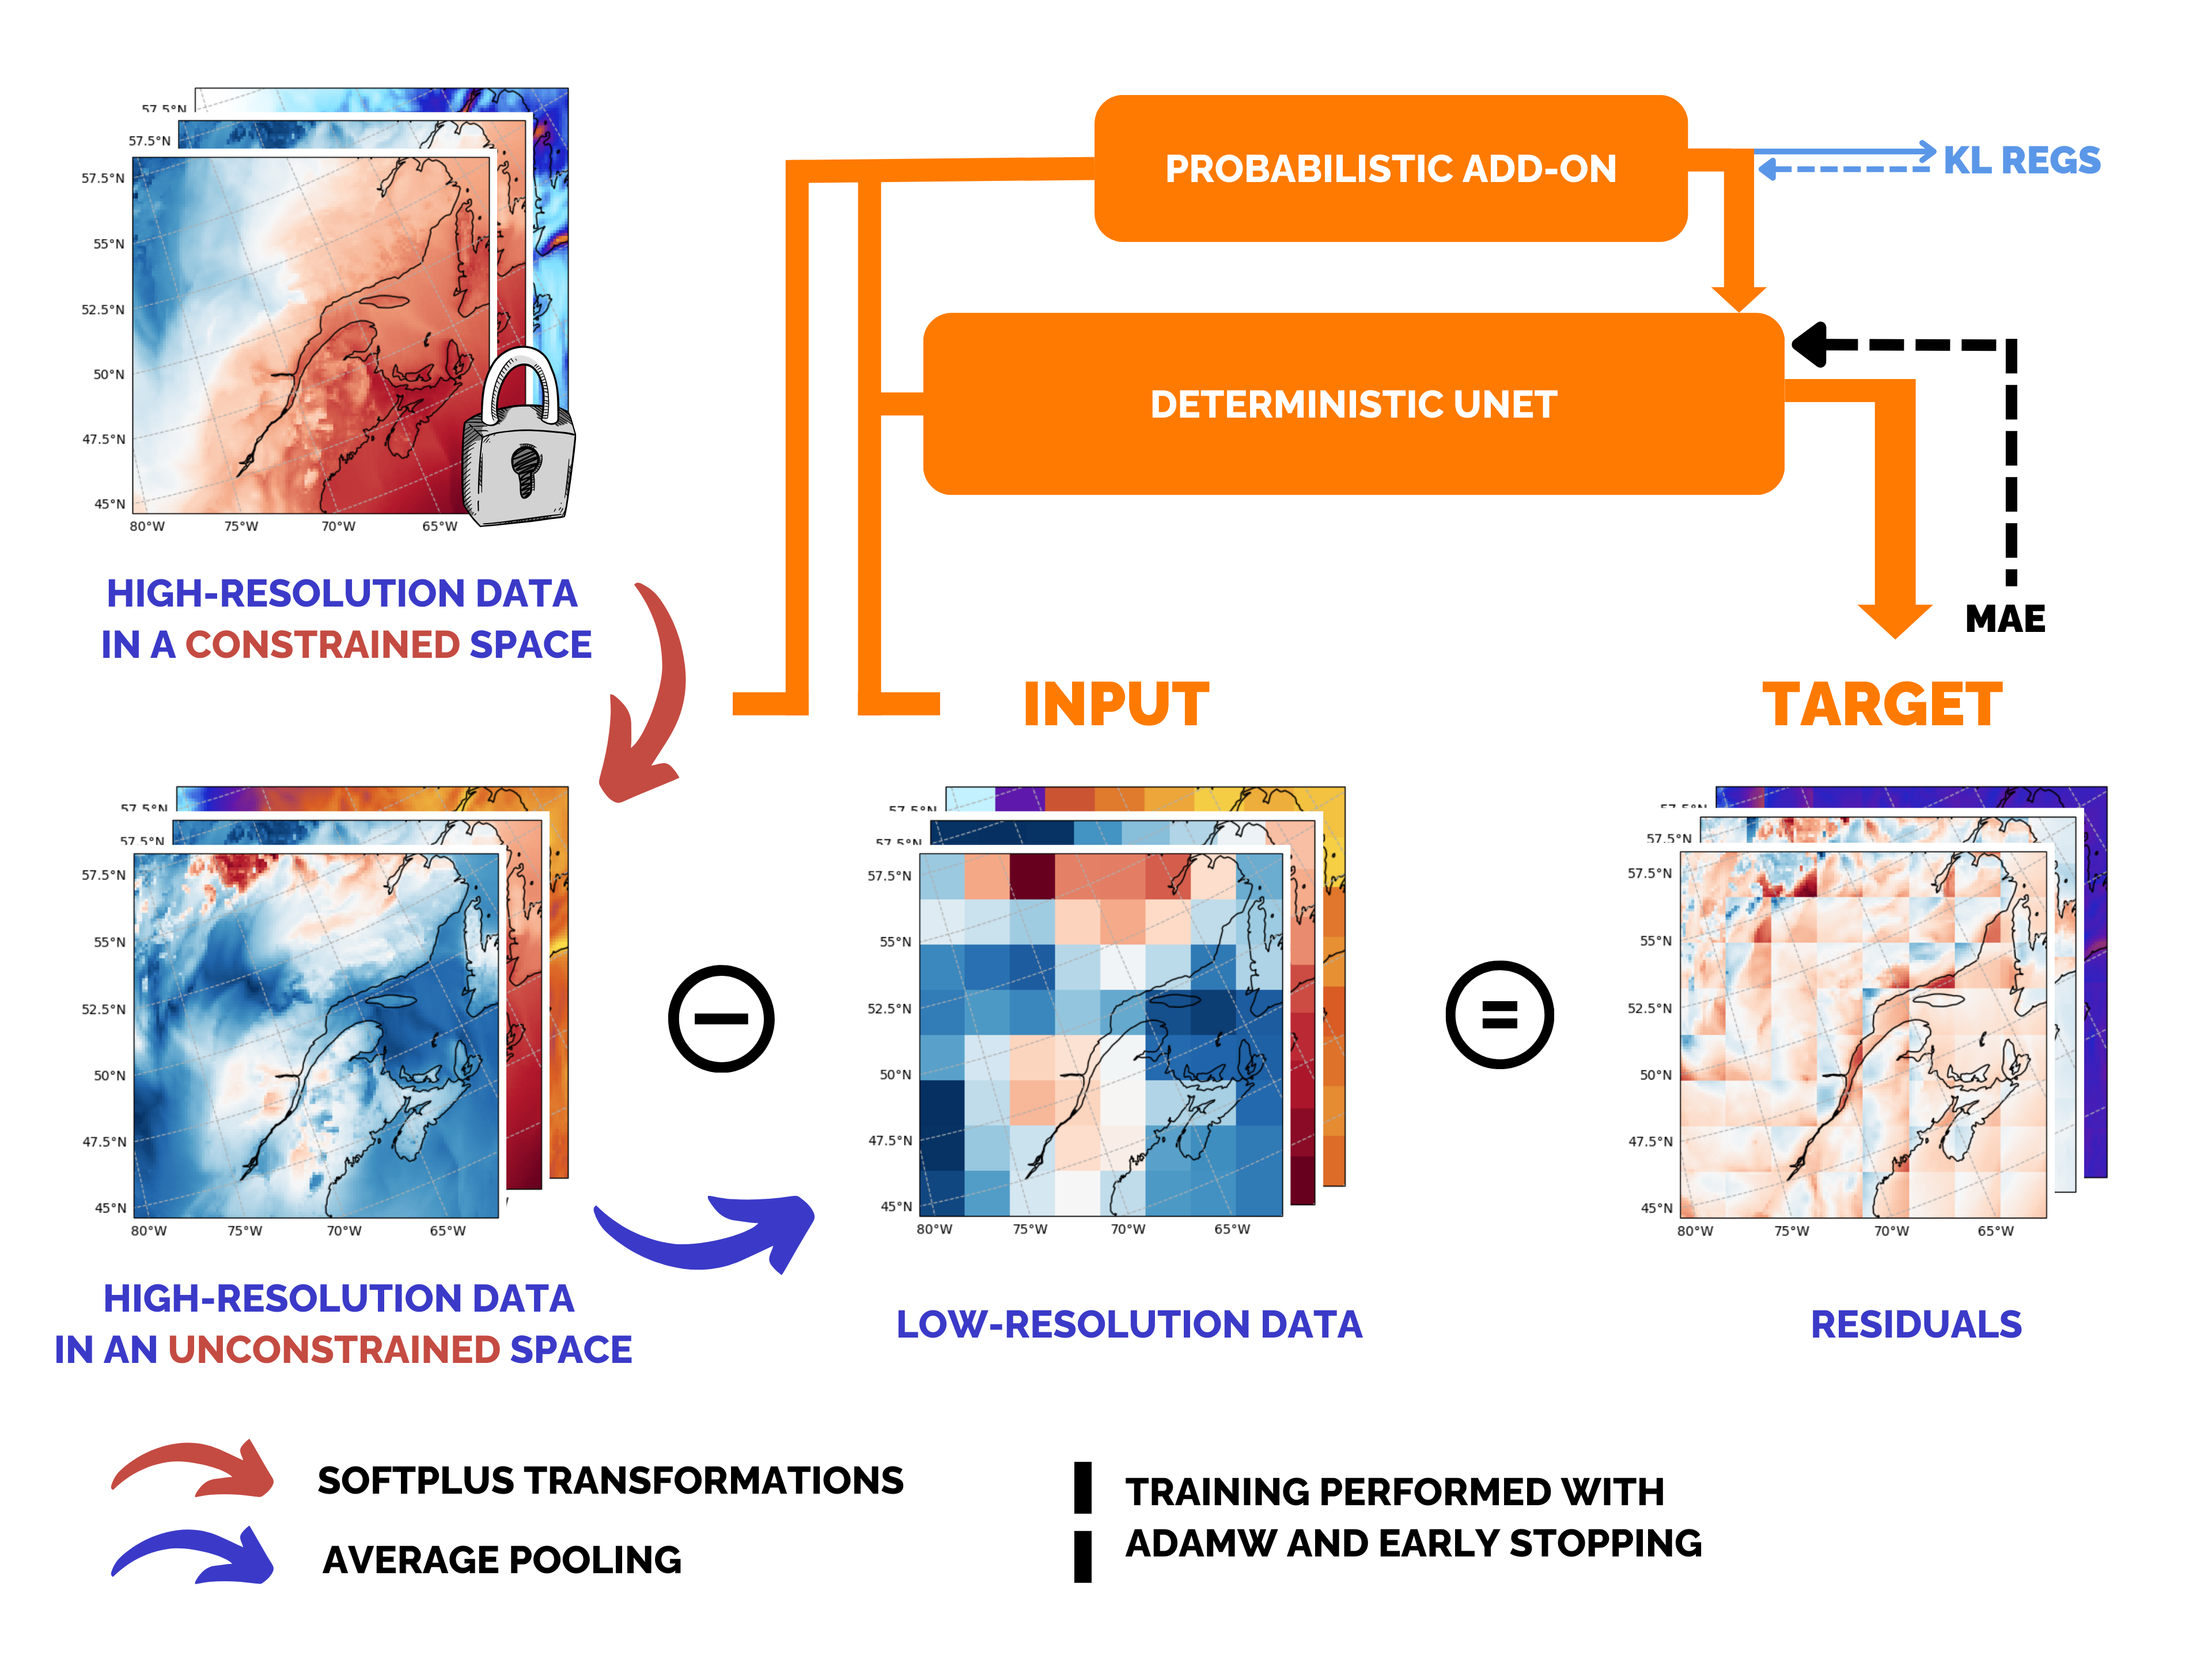
\includegraphics[width=\linewidth]{img/framework.png}
    \end{figure}

  \end{block}

    
  \begin{block}

  \vspace{25}
  
    \begin{figure}
        
\includegraphics[scale=0.25]{img/repo.png}
    \end{figure}
    
  \end{block}

\end{column}

\separatorcolumn

\begin{column}{\colwidth}

    \begin{block}{\textsc{Models}}

  \begin{block}{\textsc{Deterministic UNet}}

    \begin{itemize}
    \item \textbf{Architecture \cite{watt2024generative}:} 3-level encoder-decoder with skip connections between corresponding levels.
      \item \textbf{Input:} Low-resolution data ($8 \times 8$ grid) interpolated to high-resolution ($128 \times 128$ grid) using nearest-neighbor interpolation.
    \end{itemize}

    \begin{figure}
        \centering
        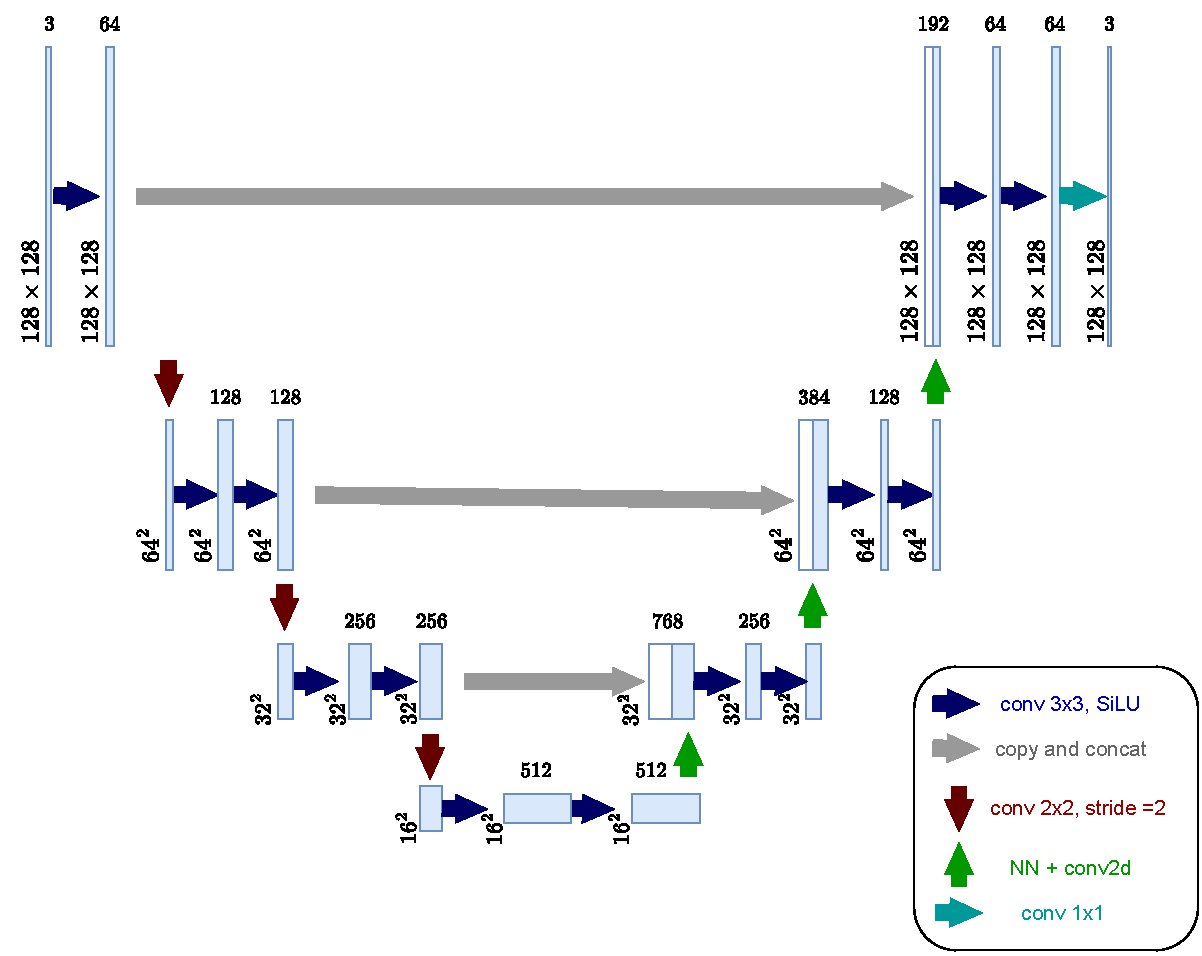
\includegraphics[scale=0.95]{img/Det-U-Net.pdf}
        % \caption{Deterministic U-Net Architecture.}
        \label{fig:architecture}
    \end{figure}


  \end{block}


  \end{block}

    \begin{alertblock}{\textsc{Probabilistic UNet}}
    The Probabilistic UNet \cite{simon2018probabilistic} incorporates a variational latent space, enabling it to model multiple plausible high-resolution outputs for a single low-resolution input.
    \heading{Components:}
    \begin{itemize}
      \item \textbf{Determisitic U-Net} 
      \item \textbf{Axis-Aligned Gaussian distribution:}  \textbf{Prior Network} &(input only&) and \textbf{Posterior Network} &(input + target&)
      \item \textbf{Loss Function:}
\[
\mathcal{L}_{\text{ELBO}} = \text{MAE}(y, \hat{y})  
\]
\[
+ \beta_1 \cdot \mathbb{E}_{q(z|x, y)} \left[ \text{KL}(q(z|x, y) \| p(z|x)) \right]
\]
\[
+ \beta_2 \cdot \mathbb{E}_{q(z|x, y)} \left[ \text{KL}(q(z|x, y) \| \mathcal{N}(0, I)) \right]
\]


% \[
% \text{MAE}(y, \hat{y}) = \frac{1}{N} \sum_{i=1}^N \frac{1}{d} \sum_{j=1}^d \left| y_{i, j} - \hat{y}_{i, j} \right|
% \]

% \[
% \text{KL}(q \| p) = \int q(z) \log \frac{q(z)}{p(z)} dz
% \]

    \end{itemize}
 \end{alertblock}
 \begin{exampleblock}
          
    % \begin{figure}
    %     \centering
    %     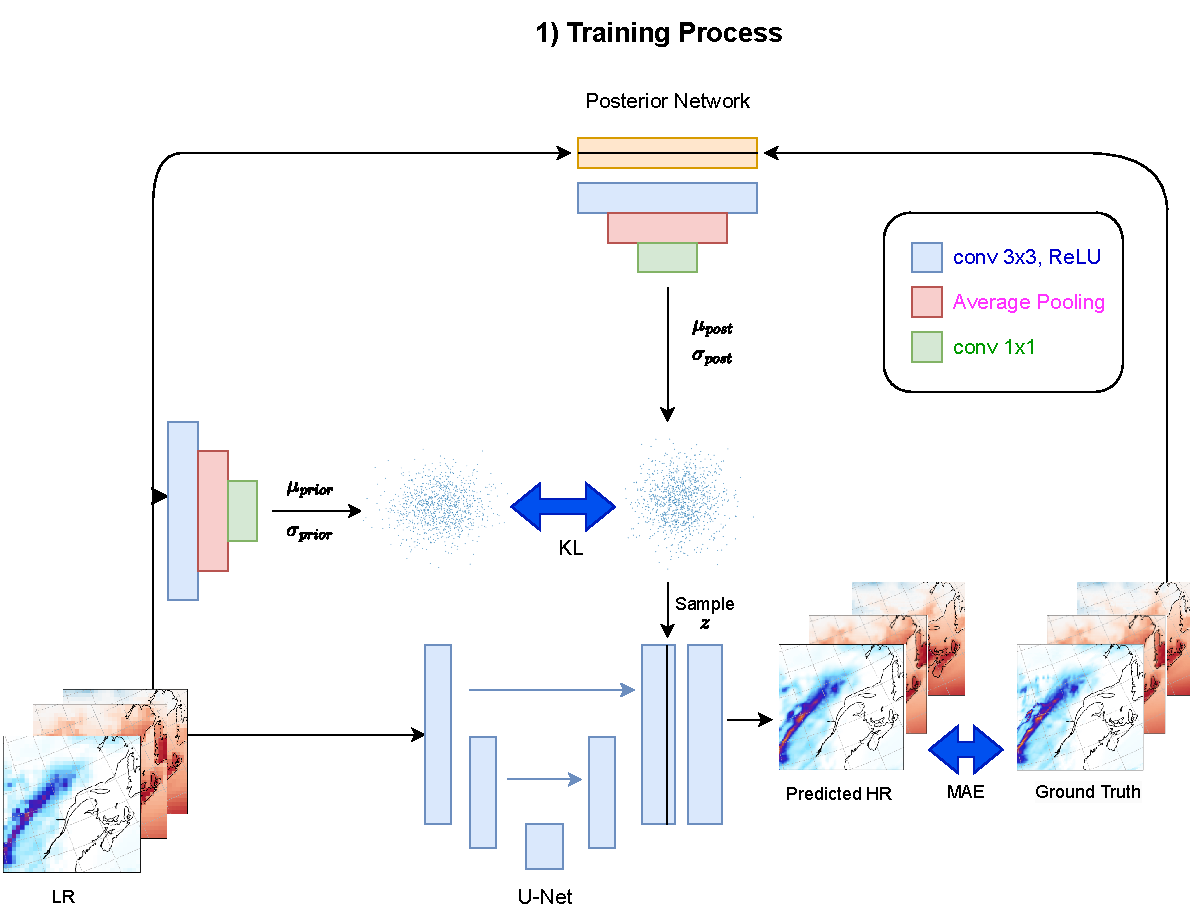
\includegraphics[width=\linewidth]{img/Prob-U-Net-training.pdf}
    %     % \caption{Training Process}
    %     \label{fig:architecture}
    % \end{figure}
    
    % \begin{figure}
    %     \centering
    %     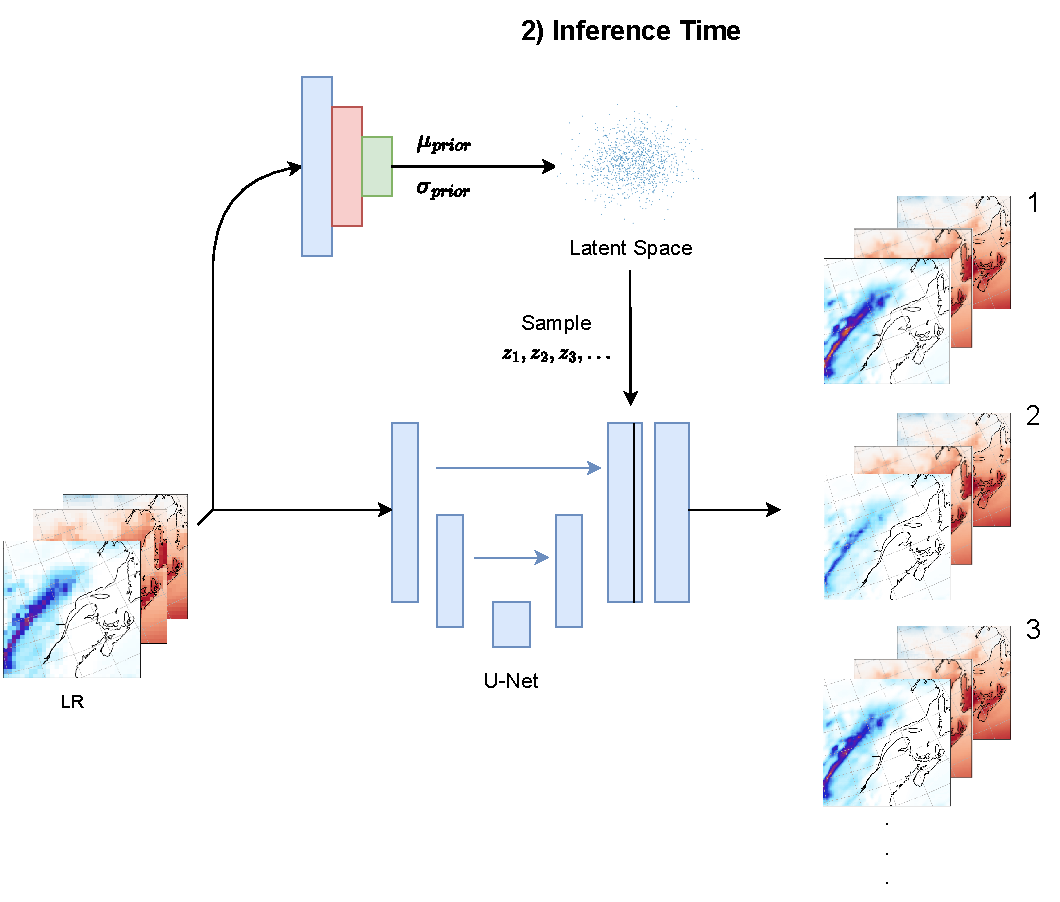
\includegraphics[width=\linewidth]{img/Prob_u-net-inference.pdf}
    %     % \caption{Training Process}
    %     \label{fig:architecture}
    % \end{figure}
    \begin{figure}
        \centering
        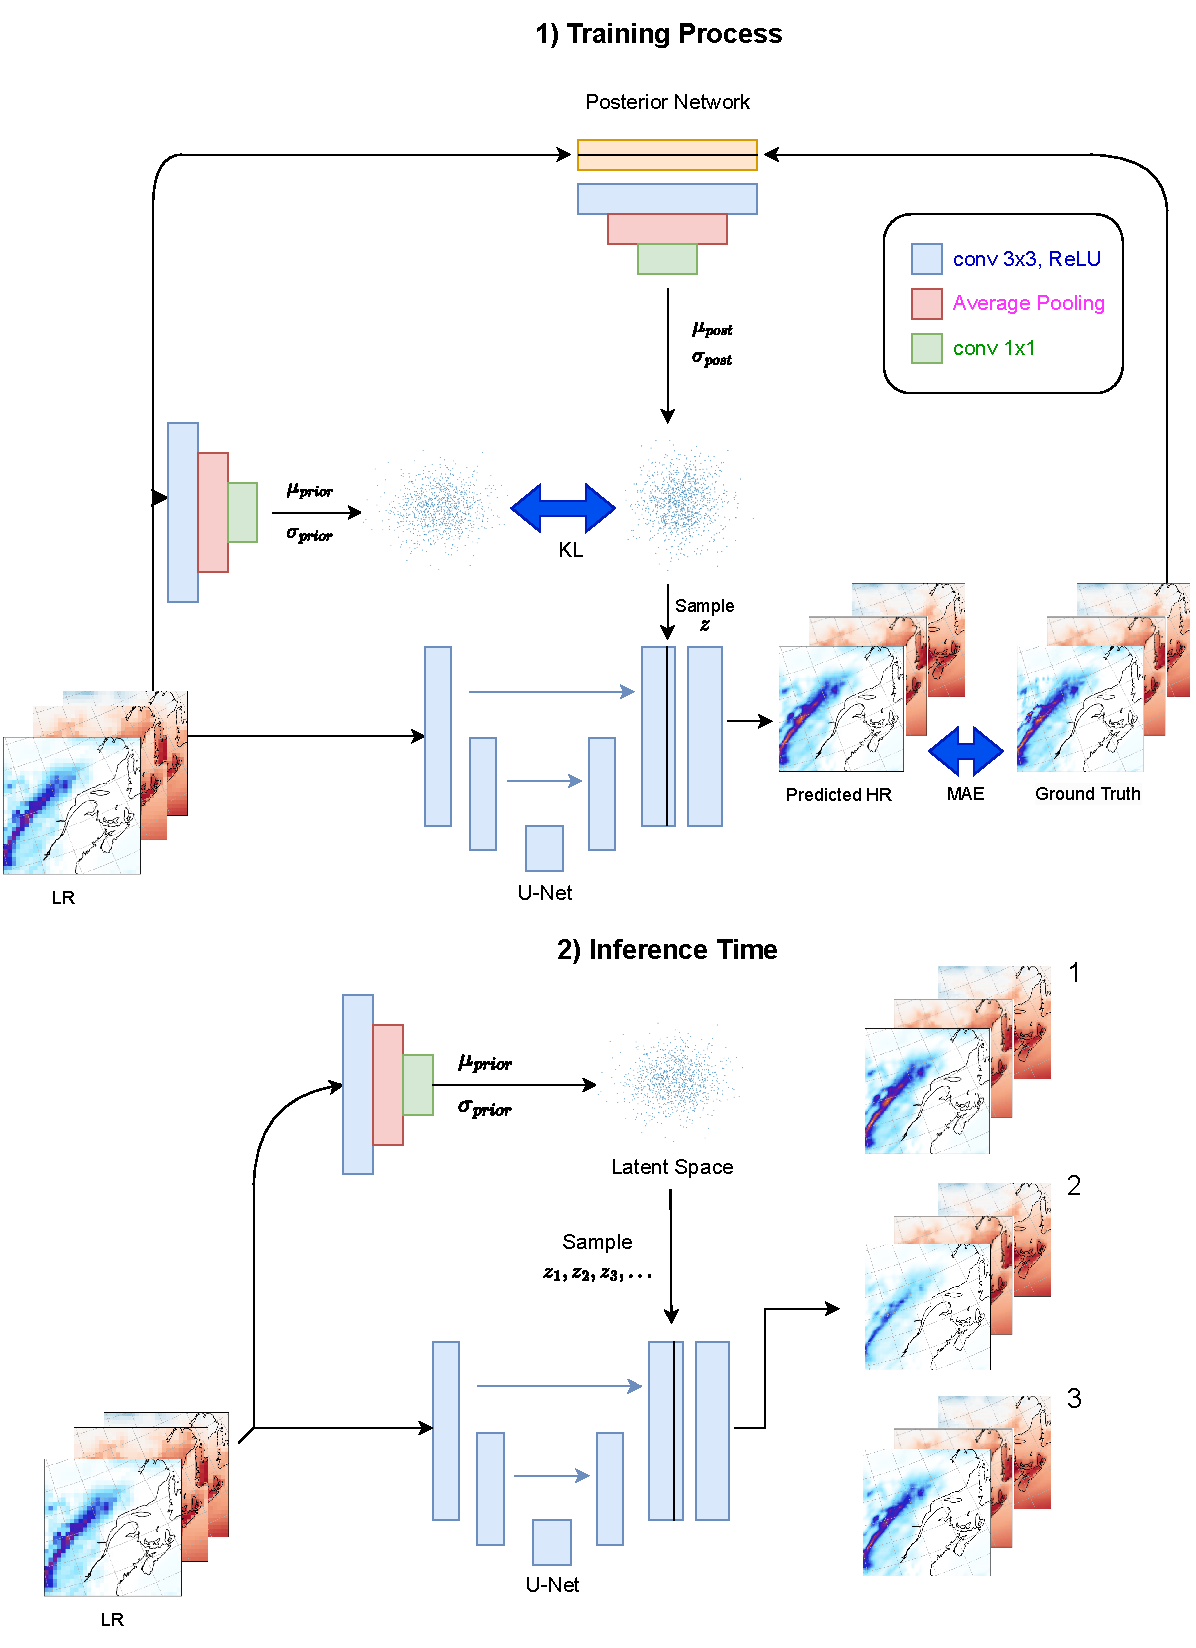
\includegraphics[width=\linewidth]{img/Prob-U-Net.pdf}
        % \caption{Training Process}
        \label{fig:architecture}
    \end{figure}
 \end{exampleblock}

\end{column}

\separatorcolumn

\begin{column}{\colwidth}

  \begin{block}{\textsc{Results and Findings}}

    \begin{figure}
        \centering
        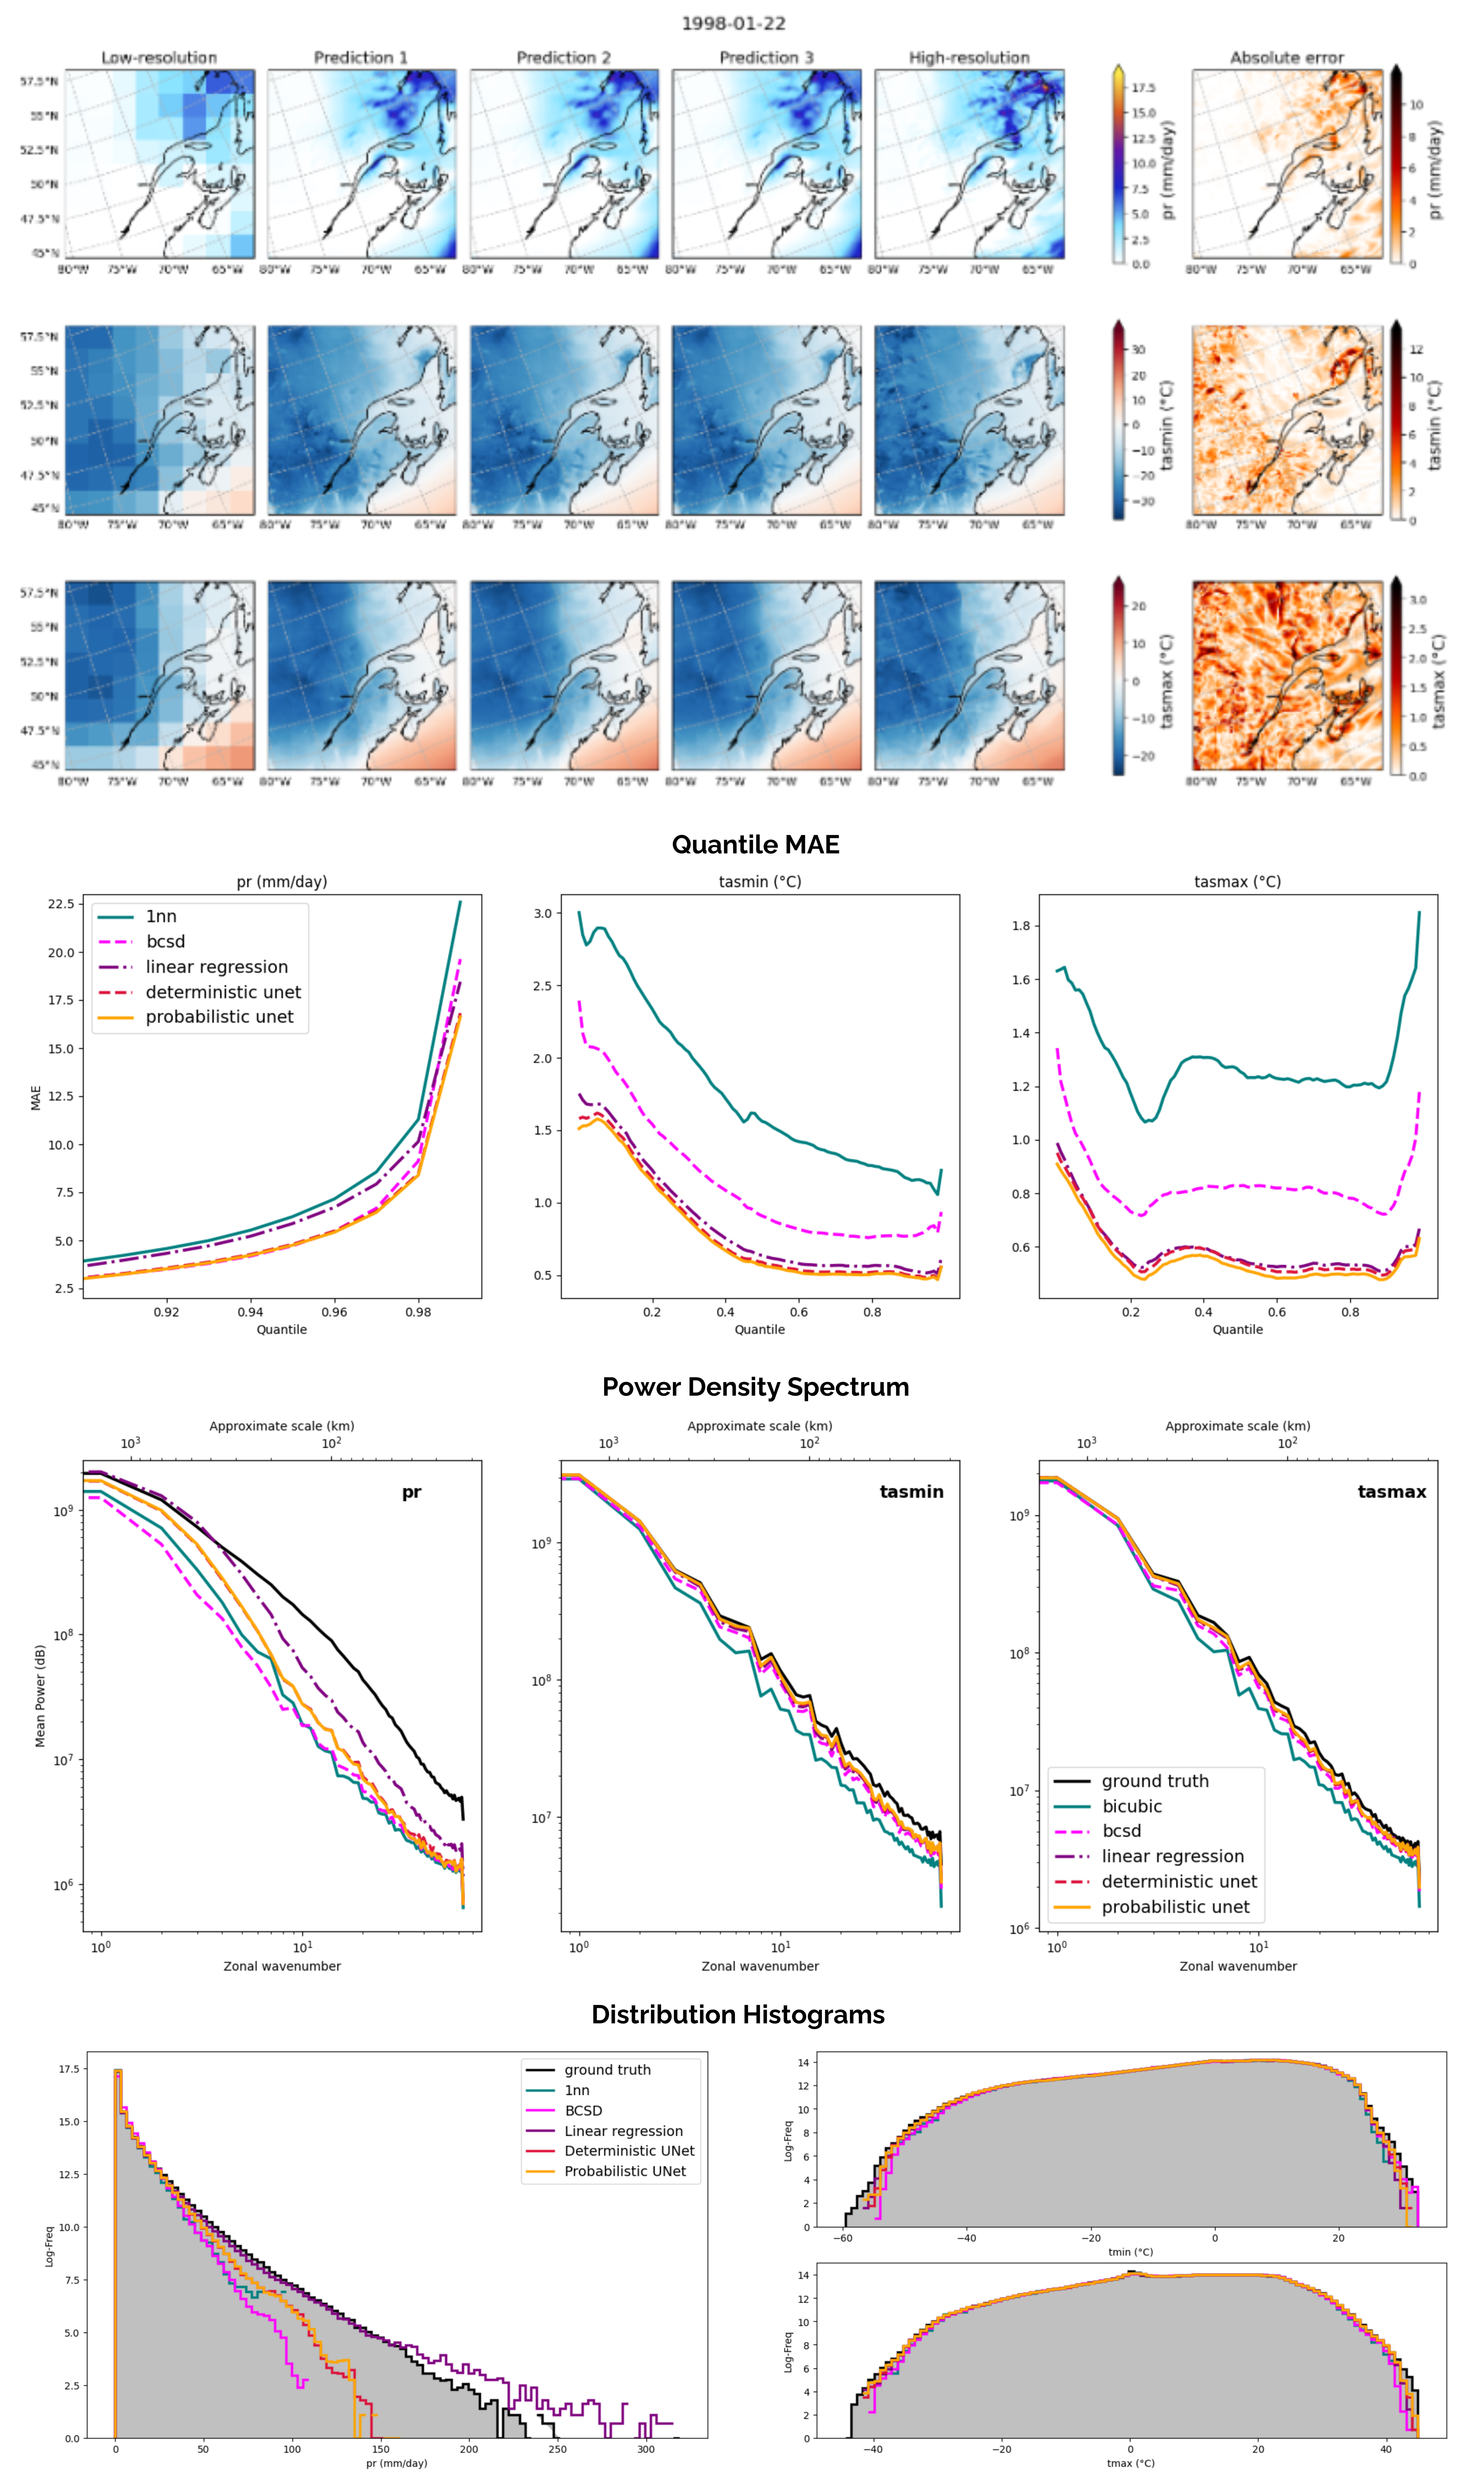
\includegraphics[width=\linewidth]{img/results.png}
    \end{figure}

    \begin{itemize}
        \item Applying \texttt{softplus} transformations to train in an \textbf{unconstrained} space avoids any \textbf{incoherent} predictions and improves performance.
        \item Predicting the \textbf{residuals} leads to \textbf{better} results regarding point-wise metrics.
        \item \textbf{Linear regression} poses as an \textbf{effective} and powerful comparative approach.
        \item Our current \textbf{probabilistic} approach \textbf{lacks} the capacity to learn and generate \textbf{diversity}.
    \end{itemize}

  \end{block}

  \begin{block}{\textsc{Next Steps}}

    \begin{itemize}
        \item Incorporate\textbf{ additional input features} (elevation, humidity, wind, geopotential, land-sea mask) into our framework.
        \item Investigate the success of linear regression.
        \item Revise the probabilistic add-on and improve its capacity \textbf{through hierarchical sampling} \cite{kohl2019hierarchical}.
        \item Explore probabilistic loss functions.
    \end{itemize}
      
  \end{block}

    \begin{block}{References}

    \nocite{*}
    \footnotesize{\bibliographystyle{plain}\bibliography{poster}}

  \end{block}
    
\end{column}

\separatorcolumn
\end{columns}
\end{frame}

\end{document}
